\documentclass[11pt]{article}
\usepackage[spanish]{babel}
\usepackage[T1]{fontenc}
\usepackage[utf8]{inputenc}
\usepackage{tikz-timing,multirow,tgheros,graphicx,fancyhdr,lscape,pdflscape,pgf,tikz}

% font
\renewcommand{\familydefault}{\sfdefault}

% biblio
\usepackage[backend = biber,style = numeric, sorting = none]{biblatex}
\addbibresource{biblio.bib}

% page setting
\usepackage[letterpaper,margin=1in]{geometry}

% tikz-timing settings
\usetikztiminglibrary[rising arrows, arrow tip=latex]{clockarrows}

% footer/headings settings
\pagestyle{fancy}
\fancyfoot[C]{}
\fancyfoot[R]{\thepage}
\fancyfoot[L]{Documentación RV32I}
\fancyhead[L,C,R]{}
\renewcommand{\footrulewidth}{0.4pt}
\renewcommand{\headrulewidth}{0pt}

\newcommand{\manualtitle}[3]{
    \begingroup
        \centering
        \vspace*{2\baselineskip}
    {\Huge\textbf{#1}}\vspace*{.4\textwidth}\par
    {\Large #3}\par\vspace*{3\baselineskip}
    
\includegraphics[width=.33\linewidth]{riscv_logo.png}\vfill
#2\par\vspace*{\baselineskip}
        \endgroup
        \newpage
}

\begin{document}
\thispagestyle{empty}
\manualtitle{Implementación de un procesador RISC-V}{Noviembre 2022}{Sebastián Nava López (ESCOM-IPN)}

\section{Introducción}
\setcounter{page}{1}

En este documento se encuentra la documentación de la implementación del procesador
RISC-V bajo el set de instrucciones RV32I en dos tipos de ejecución: ciclo sencillo
(\textit{single-cycle}) y con pipeline. Adicionalmente se incluyen detalles sobre cada
una de las unidades que forman la micro-arquitectura y se habla sobre la
demostración desarrollada a partir de la implementación de este procesador.
Mientras que la implementación con ciclo sencillo solo cubre las instrucciones
de tipo I (excepto OP = 103), R, S/B y J, el diseño con pipeline cubre el total
de las instrucciones de RV32I.

\section{Simulación}

El testbench del procesador puede ser corrido utilizando el comando
\textit{run} del Makefile incluido en el código de la implementación i.e. \textit{make run}. Los
parámetros para correr esta simulación se encuentran definidos en la constante
\verb%GHDLRUNFLAGS%.

\section{Micro-arquitectura}

\subsection{Control de saltos}
\subsubsection{Descripción}

Esta unidad tiene el objetivo de controlar la señal \verb%wpcSel% de tal forma
que, dependiendo del tipo de instrucciones que se encuentren en las etapas de
decodificación(IF/ID) y ejecución(ID/EX), así como el estado actual de la
unidad de predicción (Unidad de predicción de saltos), se tome la siguiente instrucción de
alguna de las cuatro señales disponibles en el multiplexor controlado por
\verb%wpcSel%. El algoritmo para elegir cada señal se encuentra descrito a
continuación:

\begin{verbatim}
    if jmpD:                     # Salto incondicional (jal,jalr) en IF/ID
        wpcSel := `00'           # PC = PCtargetD 
        flushD := `1'            # Descartar la instrucción que pasa de FETCH -> IF/ID 
    if brD and takeD:            # Salto condicional anticipado (inst. tipo B) cuando
                                 # el predictor (takeD) = '1'
        wpcSel := `00'           # PC = PCtargetD
        flushD := `1'
    if brE and (¬takeE and brE): # Salto condicional (instr. tipo B) en ID/EX donde 
                                 # el predictor fue negativo (takeD = '0') en IF/ID 
                                 # pero se cumple la condición de salto (breE = '1') 
        wpcSel := `01'           # PC = PCtargetE 
        flushE := `1'            # Descartar la instrucción que pasa de IF/ID -> ID/EX
        flushD := `1'
    if brE and (takeE and ¬brE): # Salto condicional en ID/EX donde el predictor  
                                 # fue '1' en IF/ID pero la condición de salto no se
                                 # cumple(breE = '0')
        wpcSel := `11'           # PC = PCplus4E
        flushE := `1'
        flushD := `1'
    else:                        # Tomar la instrucción siguiente
        wpcSel := `10'           # PC = PCplus4F
\end{verbatim}

\subsection{Unidad de Predicción de Saltos}

\subsubsection{Descripción}

La unidad de predicción de saltos es una máquina de estados finitos basada en el
diseño propuesto en el libro de \citeauthor{patterson2020computer} mostrado en
la figura \ref{fig:predictor-fsm}. Esta unidad toma 
como entrada la señal \verb%bre% de la unidad evaluadora de
condiciones y genera la señal \verb%take% que indica sí la predicción de que
la condición del salto condicional (instrucción tipo B) se va a cumplir o no. 

\begin{figure}[ht]
    \centering
    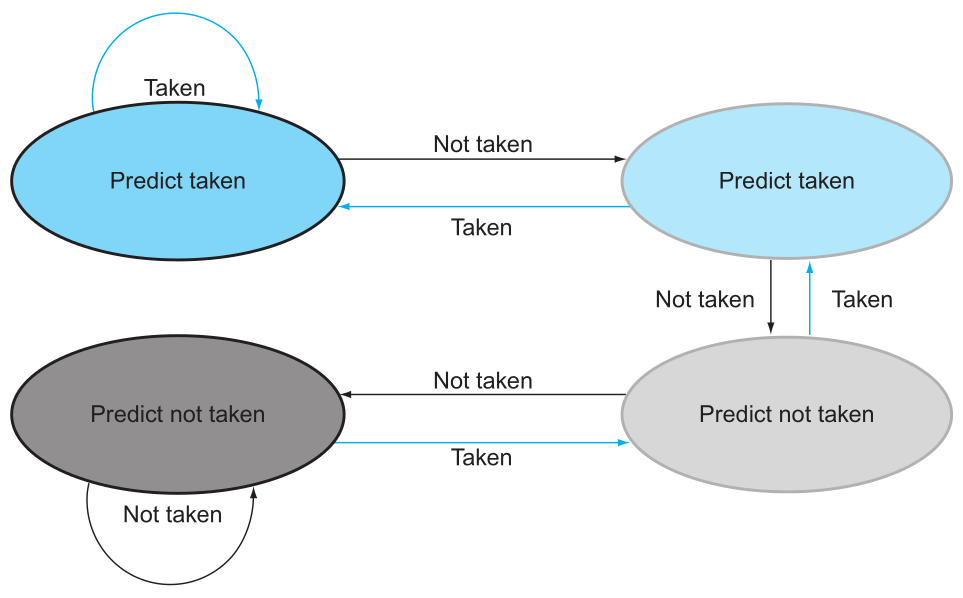
\includegraphics[width=.7\linewidth]{predictor-fsm.png}
    \caption{Maquina de estados finitos (FSM) de la unidad de predicción 
    (tomado de \citetitle{patterson2020computer} pp. 314)}
    \label{fig:predictor-fsm}
\end{figure}

\subsection{Unidad Aritmética-Lógica(ALU)}

\subsubsection{Descripción}

Unidad para realizar operaciones lógicas y aritméticas que producen diferentes
banderas dependiendo del resultado de la operación.

\subsubsection{Tabla de control}

\begin{table}[h]
    \centering
    \begin{tabular}{c|c|c|c|l l}
        aluOP       & funct7\textsubscript{5}   & funct3    & Operación &  \\\hline
        \verb%00%   & \verb%x%    & \verb%x%        & ADD   & $S = A + B$ \\
        \verb%01%   & \verb%x%    & \verb%x%        & SUB   & $S = A - B$ \\
        \verb%10%   & \verb%x%    & \verb%000%      & ADD   & $S = A + B$ \\
        \verb%11%   & \verb%0%    & \verb%000%      & ADD   & $S = A + B$ \\
                    & \verb%1%    & \verb%000%      & SUB   & $S = A - B$ \\
        \verb%1x%   & \verb%x%    & \verb%001%      & SLL   & $S = A \ll B$ \\
                    & \verb%x%    & \verb%010%      & SLT   & $S = A < B$ \\
                    & \verb%x%    & \verb%011%      & SLTU  & $S = A < B$ \\
                    & \verb%x%    & \verb%100%      & XOR   & $S = A \oplus B$ \\
                    & \verb%0%    & \verb%101%      & SRL   & $S = A \gg B$ \\
                    & \verb%1%    & \verb%101%      & SRA   & $S = A \gg B$ \\
                    & \verb%x%    & \verb%110%      & OR    & $S = A \lor B$ \\
                    & \verb%x%    & \verb%111%      & AND   & $S = A \land B$ \\
    \end{tabular}
    \caption{Tabla de control para la ALU}
\end{table}

\subsection{Evaluador de condiciones}
\subsubsection{Descripción}
Unidad genera la señal \verb%bre% a partir de las señales recibidas de la ALU,
donde el valor de \verb%bre% indica que la condición se cumple o no a partir de
los valores de las banderas. La condición que se evalúa depende de \verb%funct3%.

\subsubsection{Tabla de control}

\begin{table}[h]
    \centering
    \begin{tabular}{c|l}
        funct3      & bre \\\hline
        \verb%000%  & $EQ = Z$ \\
        \verb%001%  & $NE = \neg Z$ \\
        \verb%100%  & $LT = N \oplus OV$ \\
        \verb%101%  & $GE = \neg LT$ \\
        \verb%110%  & $LTU = \neg C$ \\
        \verb%111%  & $GEU = C$ \\
        \verb%x%   & \verb%0% \\
    \end{tabular}
    \caption{Tabla de control para el evaluador de condiciones}
\end{table}

\subsection{Archivo de Registros}
\subsubsection{Descripción}
Unidad que contiene los 32 registros del procesador.

\subsubsection{Tabla de control}

\begin{table}[h]
    \centering
    \begin{tabular}{c|c|c|l}
        CLR & CLK               & WE    & Operación \\\hline
        1   & x                 & x     & Reset \\
        0   & \texttiming{2{c}} & 0     & Banco' = Banco \\
        0   & \texttiming{2{c}} & 1     & Banco[\verb%A3%] = \verb%WD3% \\
        x   & x                 & x     & RD1 = Banco[\verb%A1%] \\
            &                   &       & RD2 = Banco[\verb%A2%] \\
    \end{tabular}
    \caption{Tabla de control para el archivo de registros}
\end{table}

\subsection{Memoria de Datos (RAM)}
\subsubsection{Descripción}
Unidad encargada del almacenamiento de datos con capacidad de lectura/escritura
en byte, palabra(\textit{word}) y media-palabra(\textit{half-word}) con
extensión de signo o padding de ceros en los modos de byte y media-palabra.

\subsubsection{Tabla de control}

\begin{table}[h]
    \centering
    \begin{tabular}{c|c|c|l}
        CLK                 & WE        & funct3        & Operación \\\hline
        \texttiming{2{c}}   & \verb%1%  & \verb%000%    & bancoRAM[\verb%A%]\textsubscript{7:0} = \verb%WD%\textsubscript{7:0} \\
                            &           & \verb%001%    & bancoRAM[\verb%A%]\textsubscript{15:0} = \verb%WD%\textsubscript{15:0} \\
                            &           & \verb%x%      & bancoRAM[\verb%A%]\textsubscript{31:0} = \verb%WD% \\
        x                   & \verb%0%  & \verb%000%    & \verb%RD% = signExt(bancoRAM[Dir]\textsubscript{7:0}) \\
                            &           & \verb%100%    & \verb%RD% = zeroExt(bancoRAM[Dir]\textsubscript{7:0}) \\
                            &           & \verb%001%    & \verb%RD% = signExt(bancoRAM[Dir]\textsubscript{15:0}) \\
                            &           & \verb%101%    & \verb%RD% = zeroExt(bancoRAM[Dir]\textsubscript{15:0}) \\
                            &           & \verb%x%      & \verb%RD% = bancoRAM[Dir]\textsubscript{31:0} \\
    \end{tabular}
    \caption{Tabla de control para memoria RAM}
\end{table}

\subsection{Memoria de programa}
\subsubsection{Descripción}
Existen dos unidades que pueden ser utilizadas como memoria de programa:
\textit{InstrMem} e \textit{InstrMemProgrammable}, localizadas en el directorio
\textit{mem/instmem/}. La primera contiene diferentes programas que van desde
pruebas simples de saltos, hasta implementaciones completas de algoritmos de
ordenamiento como \textit{bubble sort}. Estos programas están escritos a partir
de la concatenación de diferentes constantes de tal forma que sea claro el
formato de la instrucción. La segunda entidad tiene la capacidad de leer un
programa desde un archivo de texto almacenado de forma local, en la computadora
donde se lleve a cabo la simulación. La dirección de este archivo tiene que ser
establecida dentro de la entidad y su formato es de una cadena en base
hexadecimal de 32 bits por cada renglón. Un ejemplo de programa que puede ser
leído por esta entidad se encuentra en el libro de
\citeauthor{harris2021digital} capítulo 7.6.3. \textit{Testbench}

\subsection{Pipelines}
\subsubsection{Descripción}
Las pipelines de las diferentes etapas del procesador están diseñadas como una
colección de registros con escritura y reset síncronos, de tal forma que exista
cada uno de estos por cada señal que pase por el pipeline mas un registro
adicional que almacena las señales de control que son pasadas a la siguiente
etapa. Todas las entidades de este tipo se encuentran en el directorio
\textit{pipes/}.

\section{Demo FPGA}

Después de que se logró comprobar el funcionamiento del procesador a partir de
los programas de prueba que fueron corridos por medio de un testbench y
verificados a partir de los resultados de la simulación, se tomo la
determinación de llevar las pruebas un paso más allá e implementar el procesador 
por medio de una tarjeta de desarrollo equipada con una FPGA, modelo Basys 3 de
Digilent. Para esta implementación se diseñaron dos unidades para controlar el arreglo de 4
display de 8 segmentos y la cruceta de botones, ambos integrados a la
tarjeta de desarrollo, de tal forma que el procesador pueda interactuar con
ellos por medio de un esquema de mapeo de memoria. El mapa de memoria se
muestra en la figura \ref{fig:memory-map}. La memoria de programa
contiene un programa que evalúa sí algún botón fue presionado y ejecuta
diferentes acciones dependiendo del botón que fue presionado. Dicho programa
hace referencia a alguna función que pueda tomar un solo número entero como
argumento, y cuyo resultado pueda ser mostrado en el display. El archivo fuente
de la memoria de programa cuenta con dos funciones que cumplen con esta 
característica: la suma del n-ésimo término, y el cálculo del n-ésimo término 
de la secuencia Fibonacci.

La forma en la que el usuario interactúa con la demostración es
la siguiente: El display muestra una cuenta inicial (usualmente 0) que puede
ser aumentada en una unidad con el botón superior (BTNU), y disminuida en una unidad con
el botón inferior (BTND). Cuando se presiona el botón derecho (BTNR), se manda
a llamar la función mencionada anteriormente y cuando la ejecución vuelve al
programa principal, se muestra el resultado de esta función en el display.
Finalmente, el switch SW0 y el botón central (BTNC) sirven para controlar la
señal RESET. El diagrama de conexión entre el procesador (RV32I-core) y los
otros periféricos se muestra en la figura \ref{fig:demo-diag}

\begin{figure}[ht]
    \centering
    \begin{tikzpicture}[scale = 2]
        \draw (0,0) rectangle (2, 4);
        \foreach \y in {1,2,3} \draw (0, \y) -- (2, \y);
        \node[font=\ttfamily, anchor=west, text justified] at (2,4) {0x00000000};
        \node[text width=4cm, text centered] (ram) at (1,3.5)
        {\textbf{RAM}\\(con K = 8 = 256B)};
        \node[font=\ttfamily, anchor=west, text justified] at (2,3) {0x000000ff};
        \node[text centered] at (1,2.5) {\textbf{...}};
        \node[font=\ttfamily, anchor=west, text justified] at (2,2) {0x40000000};
        \node[text centered] at (1,1.5) {\textbf{4xDisplay 7s}};
        \node[font=\ttfamily, anchor=west, text justified] at (2,1) {0x80000000};
        \node[text centered] at (1,0.5) {\textbf{Botones}};
        \node[font=\ttfamily, anchor=west, text justified] at (2,0) {0xffffffff};
    \end{tikzpicture}
    \caption{Mapa de memoria del diseño de demostración}
    \label{fig:memory-map}
\end{figure}

\begin{figure}[ht!]
    \centering
    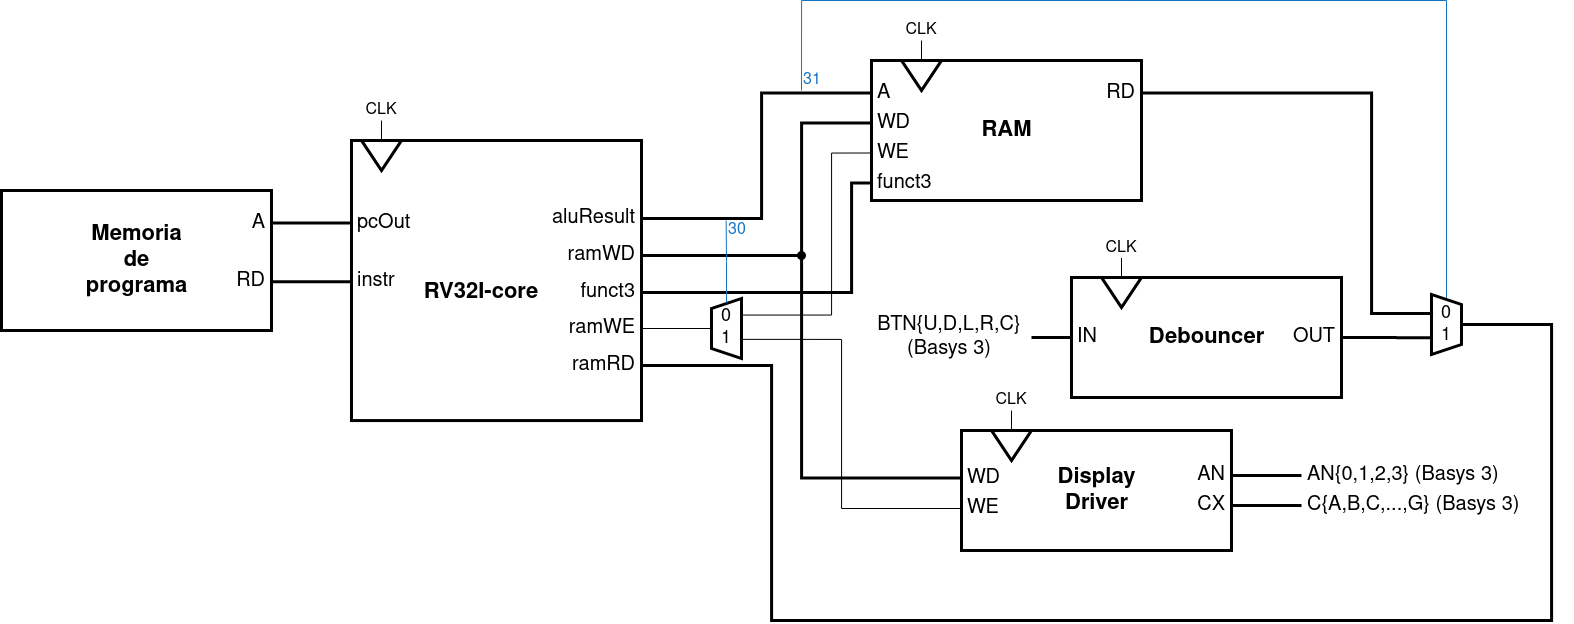
\includegraphics[width=\linewidth]{DiagramaDemo.png}
    \caption{Diagrama general del diseño de demostración}
    \label{fig:demo-diag}
\end{figure}

\begin{landscape}
    \section{Diagrama general del procesador}
    \begin{figure}[ht]
        \centering
        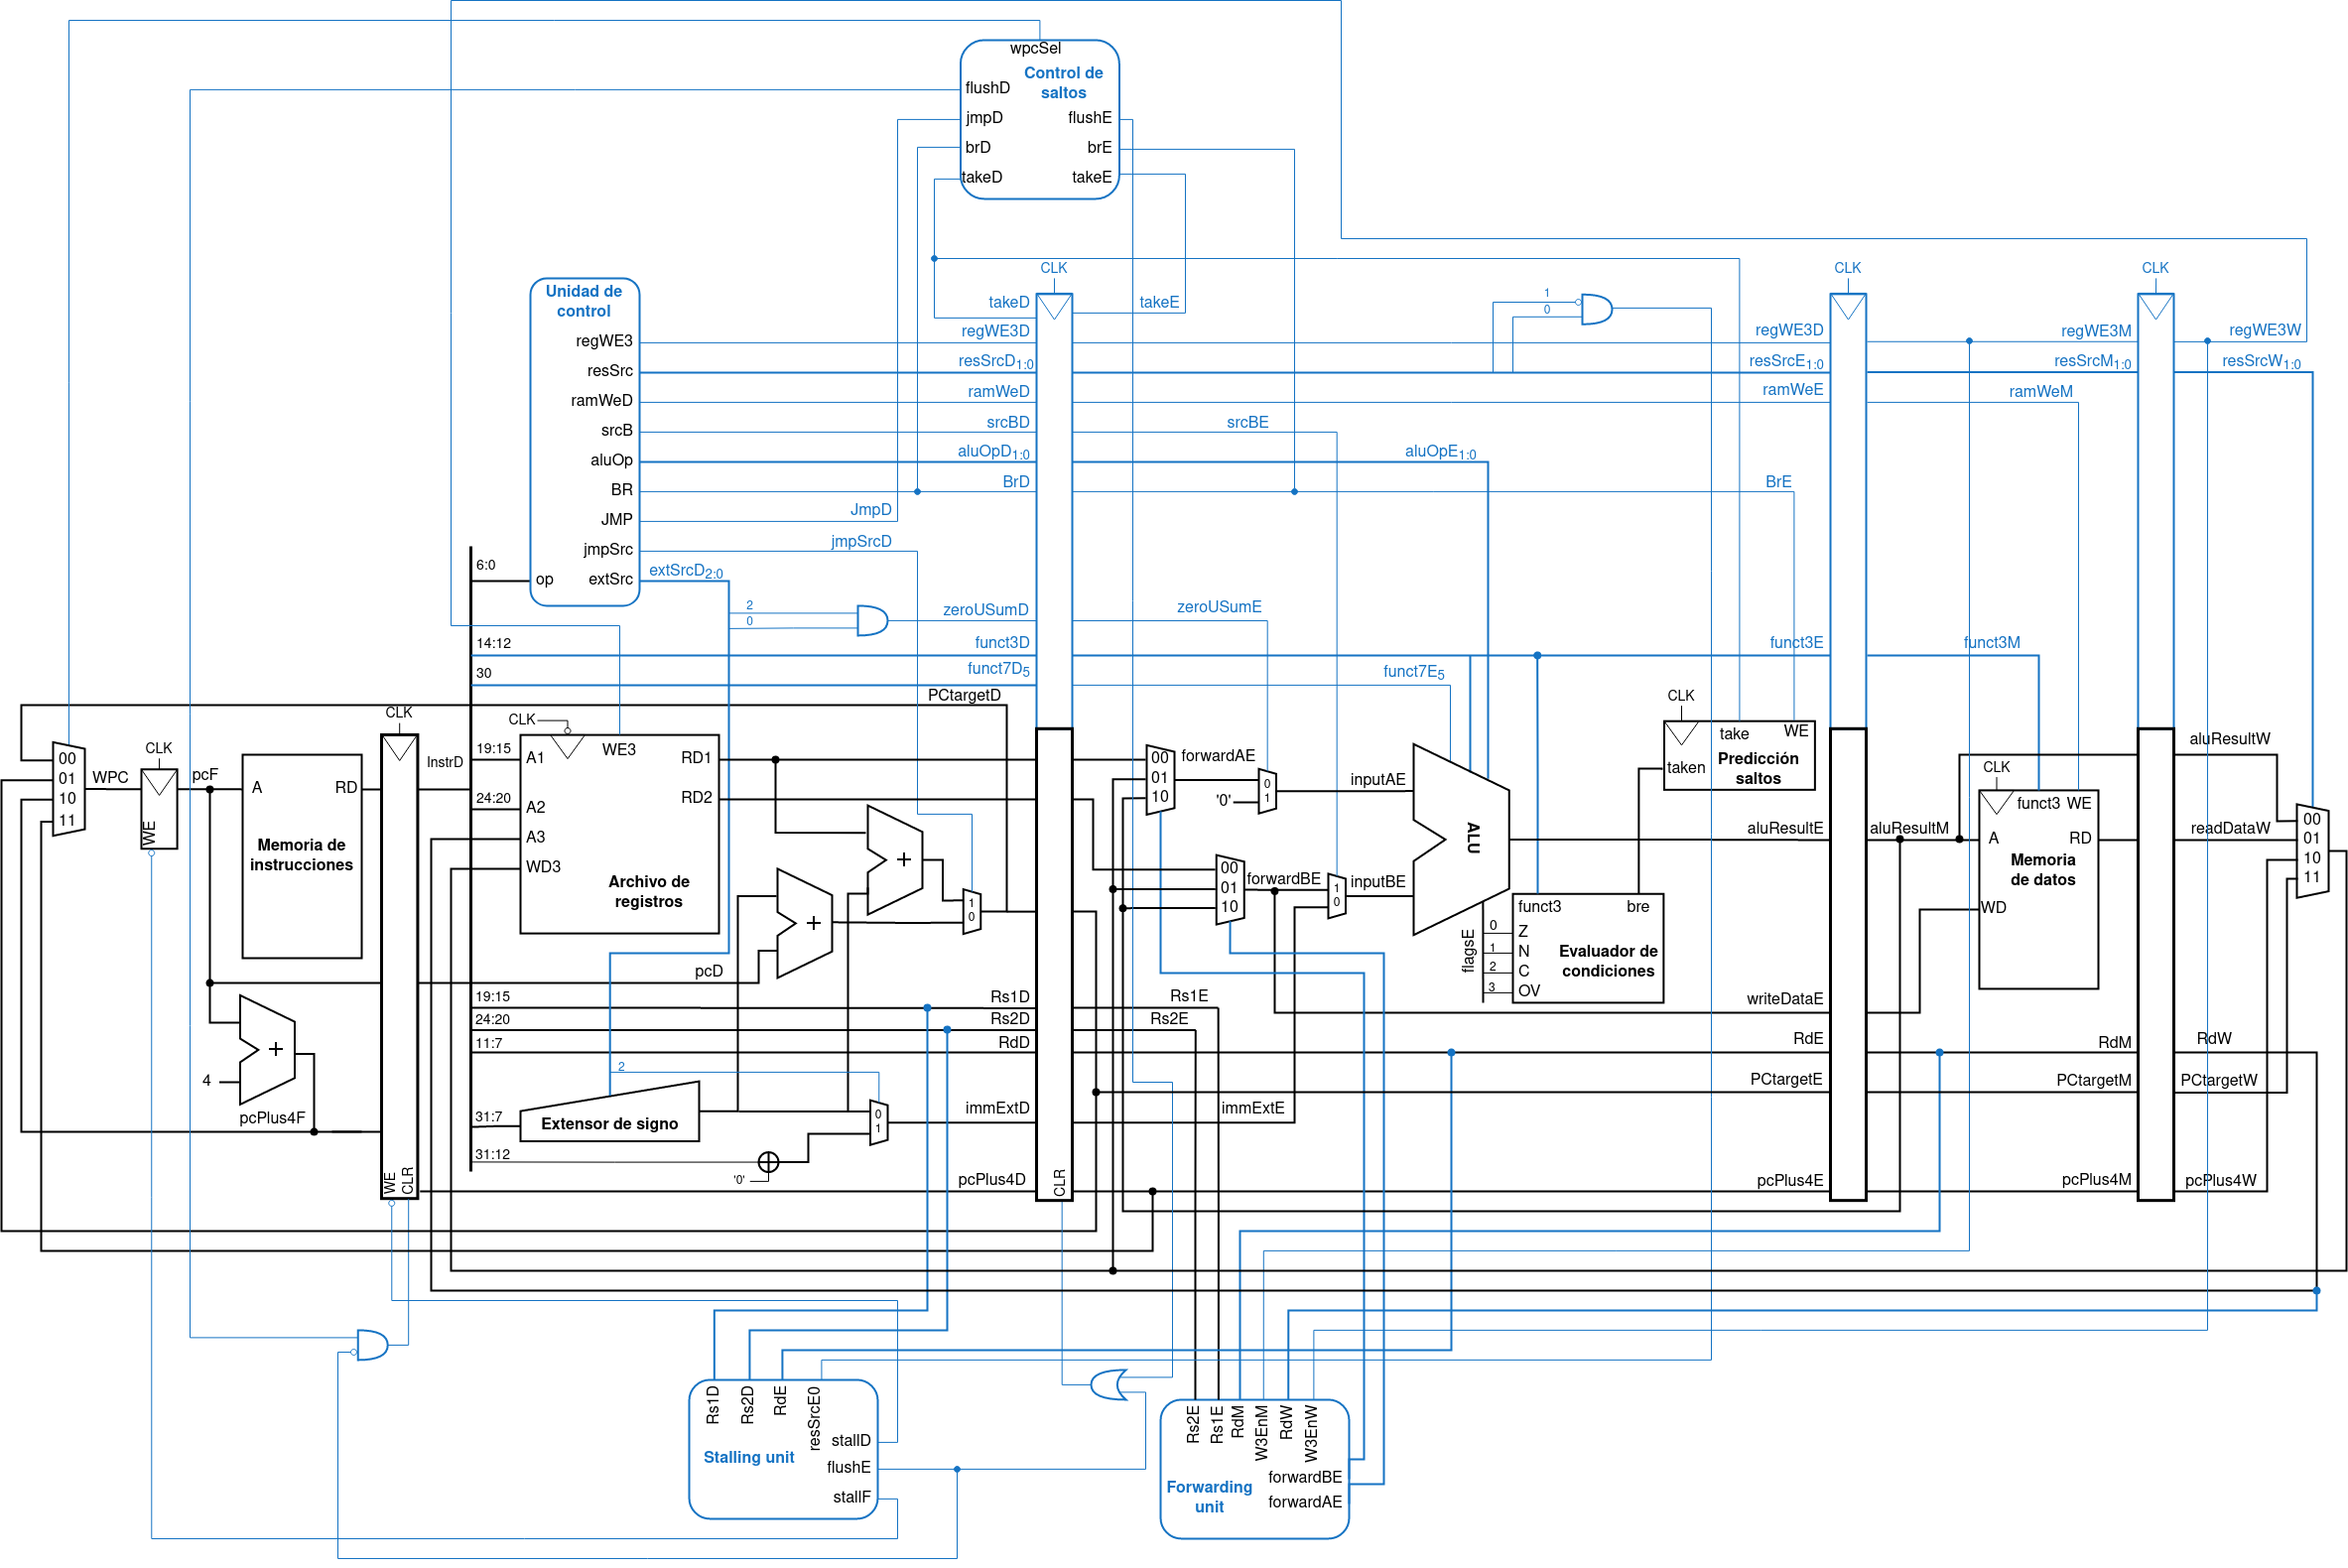
\includegraphics[width=.77\linewidth]{rv32i.png}
    \end{figure}
\end{landscape}

\printbibliography

\end{document}
